\documentclass[11pt]{standalone}

\usepackage{helvet}
\usepackage{units}
\usepackage{textcomp}

\usepackage{ifthen}
\usepackage{tikz} 
\usetikzlibrary{shapes.misc}
\usetikzlibrary{arrows,arrows.meta}
\usetikzlibrary{calc,intersections, patterns, math}
\usetikzlibrary{decorations.pathmorphing}
\usetikzlibrary{shapes.geometric}

\definecolor{pfeil}{RGB}{168,167,167}
\definecolor{petrol}{RGB}{0, 118, 136}
\definecolor{blue}{RGB}{0, 118, 136}
\definecolor{white}{RGB}{35,35,35}
% \definecolor{blue}{RGB}{100, 100, 255}
\definecolor{darkgoldenrod}{RGB}{184, 134, 11}
\colorlet{petrol-lighter}{petrol!40}
\colorlet{darkgoldenrod-lighter}{darkgoldenrod!40}
\definecolor{background}{RGB}{35,35,35}

\begin{document}

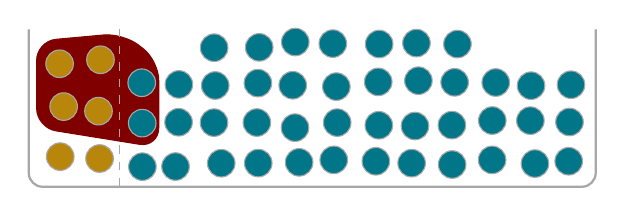
\begin{tikzpicture}[pfeil]
	\draw[thick, rounded corners=5] (-0.1,2) -- (-0.1,0) -- (7.1,0) -- (7.1,2);
			
			\draw[red!50!black, fill, rounded corners=7] (0.0,1.85) -- (0.0,0.75) -- (1.55,0.5) -- (1.55,1.6) -- (1.1,1.95) -- cycle;
			
			\foreach \x in {0.3, 0.8 }{
				\foreach  \y in {0.4,1.0,1.6}{
				\draw[fill=darkgoldenrod] ({\x+(0.5-random())*0.1},{\y+(0.5-random())*0.1}) circle (0.175);
			}
			}
			\foreach \x in {1.3, 1.8,...,6.8}{
				\foreach  \y in {0.3,0.8,1.3}{
					\draw[fill=petrol] ({\x+(0.5-random())*0.1},{\y+(0.5-random())*0.1}) circle (0.175);
				}
			}
			\foreach \x in {2.3, 2.8,...,5.3}{
				\foreach  \y in {1.8}{
					\draw[fill=petrol] ({\x+(0.5-random())*0.1},{\y+(0.5-random())*0.1}) circle (0.175);
				}
			}
			\draw[dashed] (1.05,0) -- (1.05,2);
\end{tikzpicture}




\end{document}
